\subsubsection{Total Simulation Time Scaling}
\label{subsec:total-sim-time-scaling}

Figure \ref{fig:total-sim-time-scaling} shows the total time taken to finish the simulation over the number of stations $N$ with different channel backends.
The y-axis is in logarithmic scale because the total simulation time spans more than four orders of magnitude between the smallest and largest runs.
The same results are presented in Table \ref{tab:total-sim-time-scaling}.
\begin{figure}[t]
    \centering
    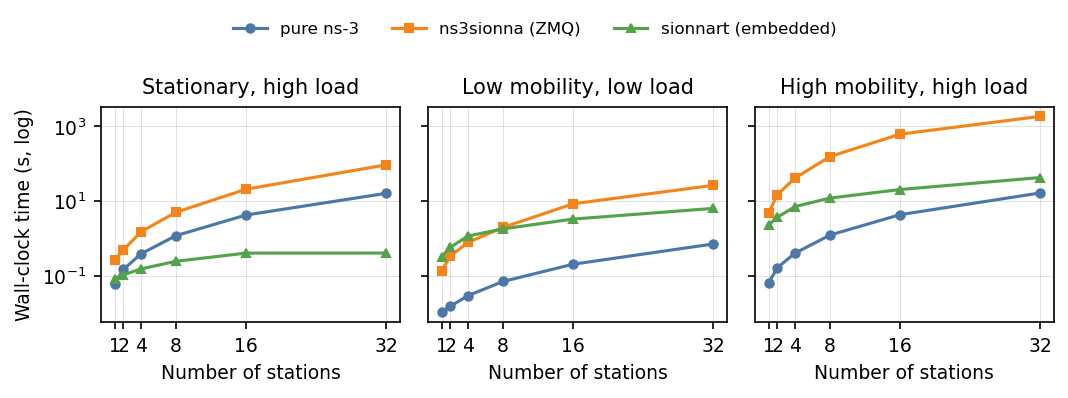
\includegraphics[width=\linewidth]{images/total-sim-time-scaling.png}
    \caption{Total simulation runtime of the three channel backends as the number of
        stations increases. The communication with external Sionna RT server via ZMQ in \texttt{ns3sionna} causes large overhead.
        The embedded \texttt{sionnart} backend avoids the round trip overhead, while the pure ns-3 baseline
        provides the analytical-channel lower bound.}
    \label{fig:total-sim-time-scaling}
\end{figure}

\begin{table}[t]
    \centering
    \caption{Total simulation runtime in seconds for representative station counts.}
    \label{tab:total-sim-time-scaling}
    \setlength{\tabcolsep}{5pt}
    \begin{tabular}{llrrrr}
        \hline
        Regime        & Backend   & $N=1$ & $N=4$  & $N=16$  & $N=32$   \\
        \hline
        Stationary    & pure ns-3 & 0.061 & 0.385  & 4.230   & 16.160   \\
        Stationary    & ns3sionna & 0.266 & 1.504  & 20.826  & 93.834   \\
        Stationary    & sionnart  & 0.082 & 0.152  & 0.403   & 0.404    \\
        \hline
        Low mobility  & pure ns-3 & 0.010 & 0.029  & 0.203   & 0.708    \\
        Low mobility  & ns3sionna & 0.137 & 0.778  & 8.453   & 26.439   \\
        Low mobility  & sionnart  & 0.320 & 1.153  & 3.292   & 6.370    \\
        \hline
        High mobility & pure ns-3 & 0.064 & 0.400  & 4.320   & 16.516   \\
        High mobility & ns3sionna & 4.821 & 41.312 & 622.365 & 1871.600 \\
        High mobility & sionnart  & 2.293 & 7.124  & 20.405  & 42.772   \\
        \hline
    \end{tabular}
\end{table}

The scaling behavior of time taken for simulation differs across different scenarios.
In the stationary scenario, the apparent advantage of \texttt{sionnart} over the \texttt{pure\_ns-3} baseline is an artefact of the cache (Section~\ref{subsec:cache-validity}), not evidence that ray-tracing is intrinsically faster than Friis evaluation.
Because no UE moves, the ray-tracer is invoked only once at $t=0$; all subsequent propagation queries are served from the cached channel snapshot while the analytical baseline still re-evaluates its loss model at every packet arrival.
This cache-driven effect produces an approximately $40\times$ wall-clock reduction at $N=32$, and would collapse to a significant overhead if mobility were introduced without the cache.
Even in this stationary scenario, \texttt{ns3sionna} backend is slower than both \texttt{pure\_ns-3} and \texttt{sionnart} backends due to the overhead of the communication between ns-3 and Sionna RT server.

In low-mobility, low-load scenario, the results show the opposite trade-off.
When the number of station counts ($N$) are low, \texttt{sionnart} is slower than \texttt{ns3sionna} because there are few propagation queries so that the cost of the query outweight the fixed cost of the embedded Python runtime and Sionna scene.
As $N$ grows, batching and cache reuse become more effective so that by the $N=32$ the performance of \texttt{sionnart} is 4.15 times faster than \texttt{ns3sionna}.
It remains 9 times slower than the \texttt{pure\_ns-3} baseline because the traffic load is low enough that stochastic propagation model remains cheap in term of computation.

The high-mobility, high-load scenario is the most important one because it is the most realistic scenario for the next generation wireless network.
In this scenario, \texttt{ns3sionna} scales poorly with the number of stations because each cache misses require copying data between processes, waiting for a request and response between two servers, and updating the Sionna side state.
The \texttt{sionnart} backend still have to pay the price of invoking the ray-tracer for each cache miss, but it avoid the overhead of inter-process communication and keeps the cache inside the same process.
As a result, the gap between \texttt{sionnart} and \texttt{ns3sionna}  grows monotonically from 2.1 times at $N=1$ to 43.8 times at $N=32$.
